% Quick start guide
% https://latex-beamer.com/tutorials/
%
\documentclass{beamer}

% \usetheme {default}

% Theme choice:
\usetheme{Frankfurt}

% Title page details
\title {\LaTeX{} Beamer introduction}
\subtitle{Quick-start guide}
\author{latex-beamer.com}
\institute{Online Education}
\date{\today}

% Image Logo
\titlegraphic{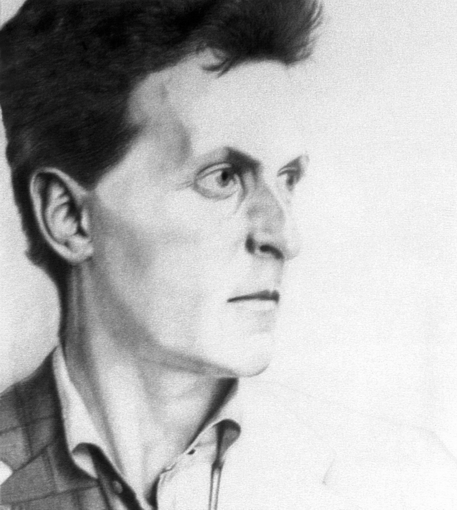
\includegraphics[width=2.5cm]{wittgenstein.png}} 

\begin{document}

\begin{frame}
% Print the title page as the first slide
\titlepage
\end{frame}

% Presentation outline
\begin{frame}{Outline}
    \tableofcontents[hideallsubsections]
\end{frame}

% Current section
\AtBeginSection[ ]
{
\begin{frame}{Outline}
    \tableofcontents[currentsection]
\end{frame}
}

% ...
% Lists in beamer (Itemize)
\begin{frame}{Lists in beamer}{Itemize environment (default)}
  \begin{itemize}

    \setbeamertemplate{itemize items}[default]
    \item First item
    \item Second item
    \item Third item
      
    \setbeamertemplate{itemize items}[circle]
    \item First item
    \item Second item
    \item Third item
      
    \setbeamertemplate{itemize items}[square]
    \item First item
    \item Second item
    \item Third item

\end{itemize}
\end{frame}

% Ordered Lists in beamer
\begin{frame}{Lists in beamer}{Enumerate environment (default)}
\begin{enumerate}
    \item First item
    \item Second item
    \item Third item
\end{enumerate}
\end{frame}

% ...
% Description Lists in beamer
\begin{frame}{Lists in beamer}{Description environment}
\begin{description}
    \item[API] Application Programming Interface
    \item[ROM] Read Only Memory
    \item[RAM] Random Access Memory
\end{description}
\end{frame}

% Tables in beamer
\begin{frame}{Simple table in beamer}
\begin{table}
\begin{tabular}{| c || c | c |}
    \hline
    No. & Name & Age \\
    \hline \hline
    1 & John T & 24 \\
    2 & Norman P & 8 \\
    3 & Alex K & 14 \\ 
    \hline
\end{tabular}
\caption{Name and age of students}
\end{table}
\end{frame}

% Figures in beamer
\begin{frame}
\begin{figure}
    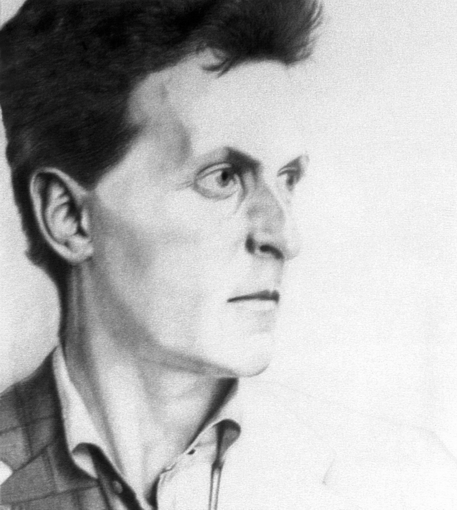
\includegraphics[scale=0.5]{wittgenstein}
    \caption{Beamer presentation}
\end{figure}
\end{frame}

% Multicolumn frame in beamer
\begin{frame}{Two columns frame in beamer}

\begin{columns}
% Column 1
\begin{column}{0.5\textwidth}
    Text here! Text here! ...
\end{column}

% Column 2
\begin{column}{0.5\textwidth}
    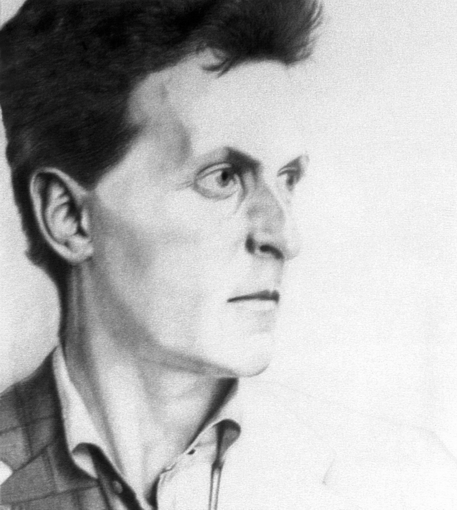
\includegraphics[scale=0.5]{wittgenstein.png}
\end{column}
\end{columns}
\end{frame}
% Blocks in beamer
\begin{frame}{Blocks in beamer}{}

\begin{exampleblock}{Block 3}
This is an example block in beamer.
\end{exampleblock}

\begin{alertblock}{Block 2}
This is an alert block in beamer.
\end{alertblock}

\begin{exampleblock}{Block 3}
This is an example block in beamer.
\end{exampleblock}
\end{frame}

% Blocks in beamer
\begin{frame}{Math related blocks in Beamer}{Theorem, Corollary and Proof}
\begin{theorem}
    It's in \LaTeX{} so it must be true $ a^2 + b^2 = c^2$.
\end{theorem}

\begin{corollary}
    a = b
\end{corollary}

\begin{proof}
    a + b = b + c
\end{proof}
\end{frame}

\end{document}
